%%===================================================================
%% Lecture 16 -- Non-Abelian SSB, Fermion Masses, and the Higgs Mechanism
%% 77609 -- Introduction to Elementary Particles
%% Date: 07/06/2026
%% Lecturer: Prof. Yonit Hochberg
%%===================================================================

\section{Lecture 16 -- Non-Abelian SSB, Fermion Masses, and the Higgs Mechanism}\label{sec:lec16}
\begin{center}
\begin{tabular}{ll}
  \textbf{Date:}\quad 07/06/2026 & \\
\end{tabular}
\end{center}
\hrule\vspace{1.5em}

%%------------------------------------------------------------------
\subsection{Overview}\label{subsec:lec16:overview}

Lecture~15 treated spontaneous symmetry breaking (SSB) of a global $U(1)$, where the entire symmetry was broken and a single Goldstone boson appeared. Today we extend the idea in three directions of increasing physical weight.

\begin{enumerate}
  \item \textbf{Non-Abelian global SSB}: a scalar triplet of $SO(3)$ acquires a vacuum expectation value (vev) that breaks $SO(3)\to SO(2)$. Only \emph{part} of the symmetry is lost, and the count of Goldstone bosons is dictated by the number of broken generators.
  \item \textbf{Fermion masses from SSB}: a chiral fermion forbidden from having a bare mass term can nevertheless become massive through a Yukawa coupling to a scalar that condenses. This is the mechanism by which every charged fermion in the Standard Model gets its mass.
  \item \textbf{The Higgs mechanism}: when the broken symmetry is \emph{local} (gauged), there is no physical Goldstone boson. Instead, the would-be Goldstone is ``eaten'' by the gauge field, which becomes massive and acquires a longitudinal polarization.
\end{enumerate}

The unifying theme is a single sentence: \emph{the vacuum, not the Lagrangian, decides which symmetries are visible in the particle spectrum}, and every broken continuous generator leaves a fingerprint --- a Goldstone boson if global, a massive gauge boson if local.

%%==================================================================
\subsection{\texorpdfstring{Non-Abelian Global SSB: $SO(3)\to SO(2)$}{Non-Abelian Global SSB: SO(3) to SO(2)}}\label{subsec:lec16:so3}

\subsubsection*{Physical Motivation}

The $SO(3)$ example is the cleanest non-Abelian generalization of last lecture's $U(1)$ because $SO(3)$ is literally the group of rotations in three dimensions. A scalar in the triplet representation can be pictured as an ordinary vector $\bvec\phi=(\phi_1,\phi_2,\phi_3)$ in an internal three-dimensional space. Giving it a vev is the same as pinning that vector to point in a definite direction. Rotations that move the vector are lost; rotations \emph{about} the vector survive. This geometric picture predicts the outcome before any algebra: a three-parameter symmetry collapses to the one-parameter group of rotations in the orthogonal plane.

\subsubsection*{Mathematical Setup}

Let $\phi_a(x)$, $a=1,2,3$, be a real scalar field in the triplet (adjoint) representation of $SO(3)$. Under an infinitesimal transformation with real parameters $\beta^a$,
\begin{equation}
  \phi \to e^{\,i\beta^a L^a}\phi,
  \qquad
  (L^a)_{bc}=-i\,\epsilon_{abc},
  \label{eq:lec16:so3_generators}
\end{equation}
where $\epsilon_{abc}$ is the totally antisymmetric Levi-Civita symbol and the $L^a$ are the three $SO(3)$ generators in the adjoint representation. The structure constants of $SO(3)$ are themselves $\epsilon_{abc}$, which is why the adjoint generators are built from them. The renormalizable, $SO(3)$-invariant Lagrangian is
\begin{equation}
  \boxed{\;\Lag
  =\tfrac12\,\partial_\mu\phi_a\,\partial^\mu\phi_a
   -\tfrac12\mu^2\,\phi_a\phi_a
   -\tfrac{\lambda}{4}(\phi_a\phi_a)^2\; ,\qquad \lambda>0\; ,}
  \label{eq:lec16:so3_lagrangian}
\end{equation}
with summation over the internal index $a$ understood. Only the rotational invariant $\phi_a\phi_a=|\bvec\phi|^2$ enters, so the potential depends solely on the length of the internal vector.

\textit{Significance:} Because the potential sees only $|\bvec\phi|^2$, the vacuum can fix the length of $\bvec\phi$ but never its direction, and that leftover directional freedom is the seed of the Goldstone bosons.

Taking $\mu^2<0$ as in the $U(1)$ case, the potential is minimized on a sphere of radius $v$ in internal space:
\begin{equation}
  \phi_a\phi_a=v^2,
  \qquad
  v^2\equiv-\frac{\mu^2}{\lambda}>0 .
  \label{eq:lec16:so3_vev_magnitude}
\end{equation}
The direction is a free choice. We exploit this freedom and align the vev entirely along the third internal axis:
\begin{equation}
  \boxed{\;\langle\phi_a\rangle=(0,0,v)\; .}
  \label{eq:lec16:so3_chosen_vacuum}
\end{equation}

\textit{Significance:} Choosing the vev to point along a single axis is a convenience, not physics --- any direction gives an equivalent spectrum, but this choice makes the residual $SO(2)$ manifest.

\begin{figure}[ht]
\centering
\begin{tikzpicture}[scale=1.0,>=stealth]
  % axes
  \draw[->] (-2.2,-0.6) -- (2.2,-0.6) node[right]{$\phi_1$};
  \draw[->] (-1.3,-1.4) -- (1.3,1.6) node[above right]{$\phi_3$};
  \draw[->] (0,-0.6) -- (1.6,0.2) node[right]{$\phi_2$};
  % vev vector
  \draw[->,very thick,blue] (0,-0.6) -- (0,1.3) node[left]{$\langle\bvec\phi\rangle=v\,\hat e_3$};
  % residual rotation in 1-2 plane
  \draw[->,myg,thick] (0.9,-0.6) arc[start angle=0,end angle=110,radius=0.9];
  \node[myg] at (0.0,0.05) {$SO(2)$};
  \fill (0,-0.6) circle (1.5pt);
\end{tikzpicture}
\caption{The vev points along $\hat e_3$ in internal space. Rotations that tilt the vector ($L^1,L^2$) are broken; the rotation about the vector ($L^3$, in the $\phi_1\phi_2$ plane) leaves it invariant and survives as $SO(2)$.}
\label{fig:lec16:so3-vev-sphere}
\end{figure}

\subsubsection*{Expansion around the Vacuum}

Shift the field by its vev, introducing fluctuations $\phi_a'$ with $\langle\phi_a'\rangle=0$. With the vev along the third axis only the third component is shifted:
\begin{equation}
  \phi_1=\phi_1',\qquad
  \phi_2=\phi_2',\qquad
  \phi_3=v+\phi_3' .
  \label{eq:lec16:so3_shift}
\end{equation}
Then
\begin{equation}
  \phi_a\phi_a
  =\phi_1'^2+\phi_2'^2+(v+\phi_3')^2
  =v^2+2v\,\phi_3'+\phi_1'^2+\phi_2'^2+\phi_3'^2 .
  \label{eq:lec16:so3_modulus_expanded}
\end{equation}
We organize the resulting Lagrangian by the number of fluctuation fields, writing $\Lag=\Lag_2+\Lag_3+\Lag_4$ (plus a constant vacuum energy and the kinetic terms, which are unaffected by the constant shift). Substituting Eq.~\eqref{eq:lec16:so3_modulus_expanded} into the potential of Eq.~\eqref{eq:lec16:so3_lagrangian} and using $\mu^2=-\lambda v^2$:

\paragraph{Quadratic terms ($\Lag_2$).}
Collect every term with exactly two fluctuation fields. From $\tfrac12\mu^2(\phi_a\phi_a)$ the quadratic part is $\tfrac12\mu^2(\phi_1'^2+\phi_2'^2+\phi_3'^2)$. From $\tfrac{\lambda}{4}(\phi_a\phi_a)^2$, squaring Eq.~\eqref{eq:lec16:so3_modulus_expanded} and keeping quadratic terms gives $\tfrac{\lambda}{4}\big[2v^2(\phi_1'^2+\phi_2'^2+\phi_3'^2)+4v^2\phi_3'^2\big]$. Adding these and using $\mu^2=-\lambda v^2$, the $\phi_1',\phi_2'$ masses cancel and only $\phi_3'$ survives:
\begin{equation}
  V_2
  =\Big(\tfrac12\mu^2+\tfrac{\lambda v^2}{2}\Big)(\phi_1'^2+\phi_2'^2+\phi_3'^2)
   +\lambda v^2\,\phi_3'^2
  =\lambda v^2\,\phi_3'^2 ,
  \label{eq:lec16:so3_quadratic_potential}
\end{equation}
so the quadratic Lagrangian and spectrum are:
\begin{equation}
  \boxed{\;\Lag_2=-\lambda v^2\,\phi_3'^2
  \;\Longrightarrow\;
  m_{\phi_3}^2=2\lambda v^2,\qquad m_{\phi_1}^2=m_{\phi_2}^2=0\; .}
  \label{eq:lec16:so3_spectrum}
\end{equation}

\textit{Significance:} The single massive mode is the radial fluctuation along the vev, while the two transverse fluctuations are exactly massless --- precisely the two Goldstone bosons demanded by the broken generators.

\paragraph{Cubic terms ($\Lag_3$).}
\begin{equation}
  \Lag_3=-\lambda v\,\phi_3'\,(\phi_1'^2+\phi_2'^2+\phi_3'^2)
  =-\lambda v\,\phi_3'\,\phi_a'\phi_a' .
  \label{eq:lec16:so3_cubic}
\end{equation}
A term proportional to $\phi_3'$ alone (selecting the third internal direction) is manifestly \emph{not} $SO(3)$ invariant: it visibly singles out the broken direction. This is a direct fingerprint of the breaking inside the Lagrangian itself.

\paragraph{Quartic terms ($\Lag_4$).}
\begin{equation}
  \Lag_4=-\frac{\lambda}{4}\,(\phi_a'\phi_a')^2 ,
  \label{eq:lec16:so3_quartic}
\end{equation}
identical in form to the unbroken quartic interaction.

\textit{Significance (of $\Lag_4$):} The dimensionless quartic coupling is untouched by SSB --- only couplings with positive mass dimension are shifted by the vev, as established last lecture.

\subsubsection*{Goldstone Counting}

This realizes Goldstone's theorem for a non-Abelian group. $SO(3)$ has three generators; the unbroken $SO(2)$ has one (the rotation in the $\phi_1\phi_2$ plane). Hence
\begin{equation}
  N_{\text{broken}}=\dim SO(3)-\dim SO(2)=3-1=2,
  \label{eq:lec16:so3_broken_count}
\end{equation}
matching the two massless scalars $\phi_1',\phi_2'$.

\cor[cor:lec16:partial-breaking]{Partial Breaking and Goldstone Count}{
When a continuous global group $G$ is spontaneously broken to a subgroup $H$, the number of Goldstone bosons equals the number of broken generators,
\begin{equation}
  N_{\text{Goldstone}}=\dim G-\dim H .
  \label{eq:lec16:goldstone_dim_count}
\end{equation}
}

\textit{Significance:} The Goldstone count is purely group-theoretic --- it depends only on how much symmetry is lost, never on the details of the potential.

\subsubsection*{The General Criterion for Broken Generators}

How do we know \emph{which} generators are broken without expanding the whole Lagrangian? The vacuum supplies the test directly. A generator $T^a$ corresponds to a broken symmetry if the group element it generates fails to leave the vacuum invariant, $e^{i\beta^a T^a}\langle\phi\rangle\neq\langle\phi\rangle$. Infinitesimally this is the statement:

\thm[thm:lec16:broken-generator-test]{Broken vs.\ Unbroken Generator}{
A generator $T^a$ is \emph{unbroken} if it annihilates the vacuum and \emph{broken} otherwise:
\begin{equation}
  \boxed{\;T^a\langle\phi\rangle=0\;\;(\text{unbroken}),
  \qquad
  T^a\langle\phi\rangle\neq 0\;\;(\text{broken})\; .}
  \label{eq:lec16:broken_generator_criterion}
\end{equation}
}

\textit{Significance:} The unbroken subgroup is exactly the stabilizer of the vacuum, so the entire symmetry-breaking pattern can be read off from a single vector $\langle\phi\rangle$.

For our example, $L^3$ generates rotations in the $\phi_1\phi_2$ plane, so $(L^3\langle\phi\rangle)_b=-i\epsilon_{3bc}\langle\phi_c\rangle=-i\epsilon_{3b3}v=0$: the third generator is unbroken. By contrast $L^1$ and $L^2$ rotate the third axis into the first and second, giving $L^{1,2}\langle\phi\rangle\neq0$, so they are broken --- consistent with the two Goldstone bosons. The homework explores further breaking patterns with this same criterion.

%%==================================================================
\subsection{Fermion Masses from Spontaneous Symmetry Breaking}\label{subsec:lec16:fermion-mass}

\subsubsection*{Physical Motivation}

In the Standard Model the left- and right-handed components of a fermion carry \emph{different} gauge charges --- they are chiral. A Dirac mass term $\bar\psi_L\psi_R$ couples the two chiralities and therefore generally violates the gauge symmetry, so it is forbidden in the Lagrangian. SSB resolves the tension: if a charged scalar condenses, the very symmetry that forbade the mass term is hidden by the vacuum, and an effective mass appears proportional to the vev. This is how electrons, quarks, and all charged fermions acquire mass.

\subsubsection*{Mathematical Setup}

Take a global $U(1)$ with a left-handed fermion $\psi_L$, a right-handed fermion $\psi_R$, and a complex scalar $\phi$ carrying charges
\begin{equation}
  q(\psi_L)=1,\qquad q(\psi_R)=2,\qquad q(\phi)=1 .
  \label{eq:lec16:yukawa_charges}
\end{equation}
A bare Dirac mass would be $\bar\psi_L\psi_R$, with net charge $-q(\psi_L)+q(\psi_R)=-1+2=+1\neq0$. It is not invariant, so
\begin{equation}
  \text{no bare mass term: }\quad \bar\psi_L\psi_R\ \text{is forbidden by }U(1).
  \label{eq:lec16:no_bare_mass}
\end{equation}
The fermions are \emph{chiral} under this $U(1)$: left and right transform differently. The only renormalizable, gauge-invariant term linking them uses the scalar --- the Yukawa coupling. Lorentz invariance pairs $\bar\psi_R\psi_L$, and charge neutrality fixes the scalar that must accompany it:
\begin{equation}
  -q(\phi^{?})+\big[-q(\psi_R)+q(\psi_L)\big]=0
  \;\Rightarrow\;
  \phi\,\bar\psi_R\psi_L\ \text{has charge}\ {+1}-2+1=0 .
  \label{eq:lec16:yukawa_charge_check}
\end{equation}
Hence the allowed interaction is
\begin{equation}
  \boxed{\;\Lag_{\text{Yuk}}
  =-y\,\phi\,\bar\psi_R\psi_L+\text{h.c.}\;,}
  \label{eq:lec16:yukawa_lagrangian}
\end{equation}
where $y$ is the dimensionless Yukawa coupling and h.c.\ denotes the Hermitian conjugate $-y^\ast\phi^\dagger\bar\psi_L\psi_R$.

\textit{Significance:} The Yukawa coupling is the unique renormalizable bridge between the two chiralities, and it is gauge invariant precisely because the scalar carries away the leftover charge that a bare mass term could not.

\subsubsection*{Generating the Mass}

Take $\mu^2<0$ so $\phi$ condenses with $|\langle\phi\rangle|=v/\sqrt2$. Choosing the vev along the real direction and expanding,
\begin{equation}
  \phi(x)=\frac{1}{\sqrt2}\big(v+h(x)+i\,\chi(x)\big),
  \qquad
  \langle h\rangle=\langle\chi\rangle=0 ,
  \label{eq:lec16:yukawa_field_expansion}
\end{equation}
with $h$ the radial (massive) fluctuation and $\chi$ the Goldstone (massless) fluctuation. Inserting into Eq.~\eqref{eq:lec16:yukawa_lagrangian},
\begin{align}
  \Lag_{\text{Yuk}}
  &=-\frac{y}{\sqrt2}\,(v+h+i\chi)\,\bar\psi_R\psi_L+\text{h.c.}
    \notag\\
  &=\underbrace{-\frac{yv}{\sqrt2}\,\big(\bar\psi_R\psi_L+\bar\psi_L\psi_R\big)}_{\text{mass term}}
    \;\underbrace{-\frac{y}{\sqrt2}\,(h+i\chi)\,\bar\psi_R\psi_L+\text{h.c.}}_{\text{scalar--fermion interactions}} .
  \label{eq:lec16:yukawa_expanded}
\end{align}
The first piece is exactly a Dirac mass linking the two chiralities into one massive Dirac fermion $\psi=\psi_L+\psi_R$:
\begin{equation}
  \boxed{\;m_\psi=\frac{y\,v}{\sqrt2}\; .}
  \label{eq:lec16:fermion_mass}
\end{equation}

\textit{Significance:} A symmetry-forbidden mass becomes allowed once the vacuum breaks the symmetry, and that mass is set by the same vev that breaks it --- mass is a measure of how strongly the fermion feels the condensate.

\begin{figure}[ht]
\centering
\begin{tikzpicture}[>=stealth]
  \coordinate (v) at (0,0);
  \draw[->,thick] (-1.6,0.9) node[left]{$\psi_L$} -- (v);
  \draw[->,thick] (v) -- (-1.6,-0.9) node[left]{$\psi_R$};
  \draw[thick,dashed] (v) -- (1.7,0) node[right]{$h,\ \chi$};
  \fill (v) circle (1.7pt);
  \node at (0.7,0.45) {$\dfrac{y}{\sqrt2}$};
\end{tikzpicture}
\caption{The Yukawa vertex after SSB. The condensate ($\phi\to v$) supplies the Dirac mass $m_\psi=yv/\sqrt2$, while the physical scalars $h$ and $\chi$ couple to the fermion with strength $y/\sqrt2=m_\psi/v$.}
\label{fig:lec16:yukawa-vertex}
\end{figure}

The interaction piece shows that the physical scalars $h$ and $\chi$ couple to the fermion with the \emph{same} coupling $y/\sqrt2$ that controls the mass. Eliminating $y$ via Eq.~\eqref{eq:lec16:fermion_mass},
\begin{equation}
  \boxed{\;g_{h\bar\psi\psi}=\frac{y}{\sqrt2}=\frac{m_\psi}{v}\; .}
  \label{eq:lec16:scalar_coupling_mass}
\end{equation}

\textit{Significance:} The scalar couples to each fermion in proportion to that fermion's mass --- a defining prediction of the Higgs boson, which interacts most strongly with the heaviest particles.

\clm[clm:lec16:vector-like]{Condition for Mass after Partial Breaking}{
In the $U(1)$ example the symmetry was broken completely. More generally, when a symmetry is only partially broken, the fermions can acquire a mass from SSB only if their representation under the \emph{unbroken} subgroup is \emph{vector-like} --- left and right components transform identically. If they remain chiral under the surviving symmetry, no invariant mass term can form.
}

\nt{After SSB the surviving Lagrangian is not the same as a theory with no symmetry at all: the broken symmetry still relates couplings (here the mass, the $h$ coupling, and the $\chi$ coupling all share the single parameter $y$). Asking for ``the $U(1)$ charge of $h$ or $\chi$'' is meaningless once the vacuum has broken the symmetry --- charge is only defined in the symmetric description.}

%%==================================================================
\subsection{\texorpdfstring{The Higgs Mechanism: SSB of a Local $U(1)$}{The Higgs Mechanism: SSB of a Local U(1)}}\label{subsec:lec16:higgs}

\subsubsection*{Conceptual Background}

Everything so far concerned \emph{global} symmetries, whose breaking produces physical massless Goldstone bosons. The decisive new feature arises when the broken symmetry is \emph{local} (gauged). A gauged symmetry has a gauge boson for each generator, and unbroken gauge bosons are necessarily massless (as $U(1)_{\rm EM}$ forces the photon to be). When such a symmetry is spontaneously broken, the gauge bosons of the broken generators \emph{gain mass}. The bookkeeping that makes this consistent is the Higgs mechanism: the would-be Goldstone boson is absorbed --- ``eaten'' --- by the gauge field and reappears as its longitudinal polarization.

\thm[thm:lec16:higgs-statement]{Higgs Mechanism (Statement)}{
Spontaneous breaking of a \emph{local} symmetry gives mass to the gauge bosons associated with the broken generators. The would-be Goldstone bosons are eaten by those gauge bosons and become their longitudinal components:
\begin{equation}
  \boxed{\;\text{broken local generator}\;\Longrightarrow\;\text{massive gauge boson}+\text{eaten Goldstone}\; .}
  \label{eq:lec16:higgs_statement}
\end{equation}
}

\textit{Significance:} Gauge symmetry forbids an explicit gauge-boson mass term, so the only way a force carrier (like the $W$ and $Z$) can be massive is for its symmetry to be spontaneously broken --- this is why mass and SSB are inseparable in the Standard Model.

\subsubsection*{Degree-of-Freedom Counting}

The mechanism is required by simple counting of physical polarizations:
\begin{itemize}
  \item A massless gauge boson has $2$ transverse polarizations.
  \item A massive vector has $3$ polarizations (two transverse, one longitudinal).
  \item A real Goldstone scalar has $1$ degree of freedom.
\end{itemize}
The total number of degrees of freedom cannot change; only their organization does:
\begin{equation}
  \boxed{\;\underbrace{2}_{\text{massless gauge}}+\underbrace{1}_{\text{Goldstone}}
  =\underbrace{3}_{\text{massive gauge}}\; .}
  \label{eq:lec16:dof_count}
\end{equation}

\textit{Significance:} The ``eaten'' Goldstone is not lost --- it is exactly the longitudinal polarization a massive vector needs, so the mechanism conserves degrees of freedom while turning a massless force carrier into a massive one.

\begin{figure}[ht]
\centering
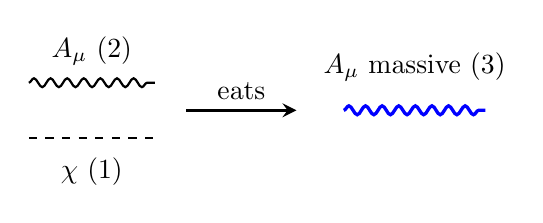
\begin{tikzpicture}[>=stealth,scale=1.0]
  % left: massless gauge + goldstone
  \draw[decorate,decoration={snake,amplitude=1.6pt,segment length=6pt},thick]
    (-3.6,0.35) -- (-2.0,0.35);
  \node at (-2.8,0.75) {$A_\mu$ (2)};
  \draw[thick,dashed] (-3.6,-0.35) -- (-2.0,-0.35);
  \node at (-2.8,-0.78) {$\chi$ (1)};
  % arrow
  \draw[->,very thick] (-1.6,0) -- (-0.2,0) node[midway,above]{eats};
  % right: massive gauge
  \draw[decorate,decoration={snake,amplitude=1.6pt,segment length=6pt},very thick,blue]
    (0.4,0) -- (2.2,0);
  \node at (1.3,0.55) {$A_\mu$ massive (3)};
\end{tikzpicture}
\caption{Higgs mechanism as degree-of-freedom rearrangement. The $2$ polarizations of the massless gauge boson plus the $1$ Goldstone scalar reorganize into the $3$ polarizations of a massive vector.}
\label{fig:lec16:higgs-dof}
\end{figure}

\subsubsection*{Mathematical Setup}

Promote the global $U(1)$ to a local one. A scalar $\phi$ of charge $+1$ transforms as
\begin{equation}
  \phi(x)\to e^{i\theta(x)}\phi(x),
  \qquad
  D_\mu\phi=(\partial_\mu+i g A_\mu)\phi ,
  \label{eq:lec16:local_u1_transformation}
\end{equation}
with $g$ the gauge coupling and $A_\mu$ the gauge field (the analog of the photon). The gauge-invariant Lagrangian is
\begin{equation}
  \boxed{\;\Lag
  =(D_\mu\phi)^\dagger D^\mu\phi
   -\frac14 F_{\mu\nu}F^{\mu\nu}
   -\mu^2\,\phi^\dagger\phi
   -\lambda\,(\phi^\dagger\phi)^2\; ,}
  \label{eq:lec16:local_u1_lagrangian}
\end{equation}
where $F_{\mu\nu}=\partial_\mu A_\nu-\partial_\nu A_\mu$ is the Abelian field strength. This differs from the global theory only by the covariant derivative and the gauge kinetic term.

\textit{Significance:} The covariant derivative is the entire source of the gauge-boson mass: when $\phi$ is replaced by its vev inside $(D_\mu\phi)^\dagger D^\mu\phi$, the term $g^2|\langle\phi\rangle|^2 A_\mu A^\mu$ is precisely a photon mass.

For $\mu^2<0$ the scalar condenses with $|\langle\phi\rangle|=v/\sqrt2$, $v=\sqrt{-\mu^2/\lambda}$, breaking the local $U(1)$. Rather than the linear (real/imaginary) split used earlier, it is now convenient to write the complex scalar in \emph{magnitude--phase} (polar) variables:
\begin{equation}
  \boxed{\;\phi(x)=e^{\,i\chi(x)/v}\,\frac{v+h(x)}{\sqrt2}\; .}
  \label{eq:lec16:nonlinear_realization}
\end{equation}
This is called the \emph{nonlinear realization} of the field: $h$ is the radial (Higgs) excitation and $\chi$ is the phase (would-be Goldstone) excitation, both with zero vev. To leading order in the phase, $e^{i\chi/v}\approx 1+i\chi/v$, so it reduces to the linear realization $\phi\approx\tfrac{1}{\sqrt2}(v+h+i\chi)$ used in Eq.~\eqref{eq:lec16:yukawa_field_expansion}.

\textit{Significance:} In the nonlinear realization the would-be Goldstone $\chi$ sits entirely in the \emph{phase}, exactly the part a gauge transformation can rotate --- which is what makes ``eating'' the Goldstone a simple change of gauge.

\subsubsection*{Outlook: Unitary Gauge}

The phase $\chi(x)$ appears only through $e^{i\chi/v}$. Because the symmetry is now \emph{local}, we are free to perform an $x$-dependent gauge rotation $\theta(x)=-\chi(x)/v$ that removes the phase entirely, leaving
\begin{equation}
  \phi(x)\ \longrightarrow\ \frac{v+h(x)}{\sqrt2}\qquad(\text{unitary gauge}).
  \label{eq:lec16:unitary_gauge_preview}
\end{equation}
The degree of freedom $\chi$ has not vanished; the same gauge transformation shifts $A_\mu$, depositing $\chi$ into the gauge field as its longitudinal mode. Carrying this through the covariant derivative produces the explicit gauge-boson mass term --- the calculation we complete next lecture (Thursday).

\nt{The contrast with the global case is sharp: for a global symmetry no gauge transformation exists to remove $\chi$, so it survives as a physical massless Goldstone boson. The locality of the symmetry is exactly what converts the Goldstone into a longitudinal polarization.}
